El transporte de jets es una herramienta conveniente por dos principales razones: la primera es que al integrar la parametrización de la vecindad de $\xo$ con polinomios de orden $M$, se pueden obtener términos variacionales hasta de este orden de manera automática. En este sentido, es importante que el transporte sea suficientemente preciso para dichas variaciones. Se prupuso en la sección \ref{sec:ximax} una forma de controlar el error del método via $\xi_{max}$. En éste apéndice se mostrará, tomando al PC3C, la precisión respecto a la integración nominal a distintos órdenes de jet y distintas condiciones inciales, con todos los demás parámetros fijos. 

%FIGURA!
\begin{figure}[h!]
\centering
\begin{subfigure}{0.49\textwidth}
	\centering
	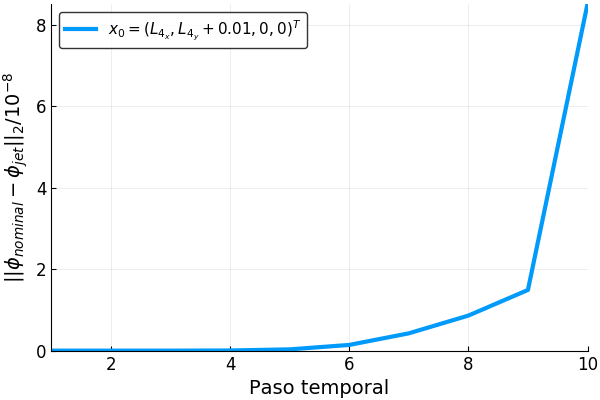
\includegraphics[width = \textwidth]{acc_c3bp_ci1}
\end{subfigure}
%
\begin{subfigure}{0.49\textwidth}
	\centering
	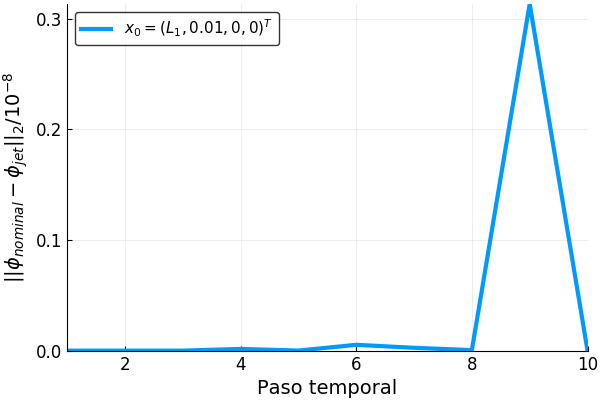
\includegraphics[width = \textwidth]{acc_c3bp_ci2}
\end{subfigure}
\caption{Diferencia entre la integración nominal y el transporte de jets para dos condiciones iniciales del PC3C con $\mu = 0.012$. Las integraciones para ambos casos fueron realizadas con una tolerancia $\epsilon_{Taylor} = 10^{-18}$, orden de la expansión $N=20$, orden del jet $M=4$ y $6$ unidades temporales a $10$ pasos de integración. \textit{Izquierda}: $\xo =\left(L_{4_x}, L_{4_y} + 0.01, 0, 0 \right)^T$. \textit{Derecha}: $\xo = \left(L_{1_x}, 0.01, 0, 0 \right)^T$.}
\label{fig:acc_ci}
\end{figure}

En la figura \ref{fig:acc_ci} se muestra cómo la precisión de las evaluaciones del jet para variaciones tamaño $\norm{\delta \xo} = \xi_{max}$ queda siempre del orden de$10^{-8}$, que es bastante inferior a la cota máxima dada $\epsilon_{jet} = 10^{-5}$. El error de la condición $x_0 = (L_{1}, 0.01, 0,0)^T$ es menor, sin embargo, el tamaño de la vecindad tuvo que ser mucho más pequeña $\xi_{max} = 2.03 \times 10^{-5}$ comparado con la otra condición inicial, donde $\xi_{max} = 2.33 \times 10^{-3}$. 

%FIGURA!
\begin{figure}[h!]
\centering
\begin{subfigure}{0.49\textwidth}
	\centering
	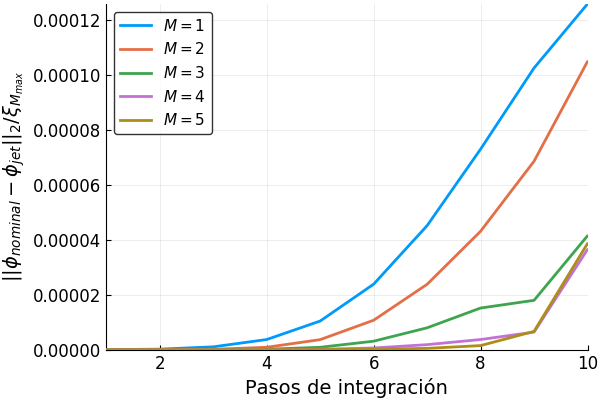
\includegraphics[width = \textwidth]{acc_c3bp_M}
\end{subfigure}
%
\begin{subfigure}{0.49\textwidth}
	\centering
	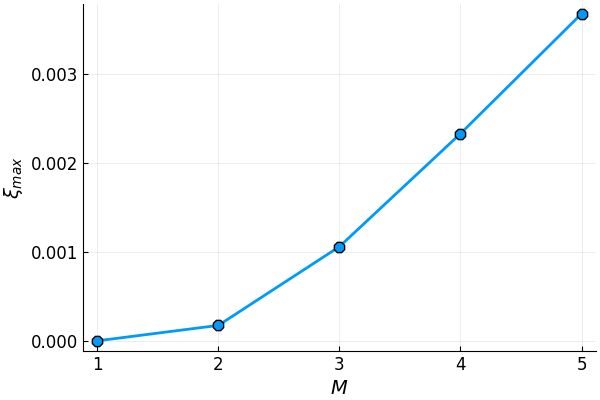
\includegraphics[width = \textwidth]{M_ximax}
\end{subfigure}
\caption{ \textit{Izquierda}: Diferencia entre la integración nominal y el transporte de jets en términos del $\xi_{max}$ correspondiente para diferentes órdenes $M$ del jet con condición inicial $\xo =\left(L_{4_x}, L_{4_y} + 0.01, 0, 0 \right)^T$. Las integraciones para ambos casos fueron realizadas con una tolerancia $\epsilon_{Taylor} = 10^{-18}$, orden de la expansión $N=20$, $\epsilon_{jet} = 10^{-5}$ y $6$ unidades temporales a $10$ pasos de integración. \textit{Derecha}: Tamaño máximo de vecindad $\xi_{max}$ para diferentes órdenes de jet con las condiciones mencionadas.}
\label{fig:acc_M}
\end{figure}

La figura izquierda de \ref{fig:acc_M} muestra la misma diferencia que \ref{fig:acc_ci} en unidades de $\xi_{M_{max}}$, donde varía el orden del jet. Se toma como condición inicial a $\xo =\left(L_{4_x}, L_{4_y} + 0.01, 0, 0 \right)^T$.  Se observa como el orden de magnitud del error sidminuye entre mayor sea el orden, aún cuando para cada caso la cantidad esté dividida entre una $\x_{max}$ mayor. A la derecha de la figura se observa cómo $\xi_{max}$ es notablemente más pequeña mientras menor es el orden utilizado. Esto quiere decir que siempre se puede obtener la misma precisión, con el precio de reducir el diámetro potencial de la vecindad inicial.

%Un último comentario sobre la precisión es, nuevamente, sobre la cantidad $\xi_{max}$. La ecuación \ref{} construye al tamaño máximo de vecindad con el supuesto de que será cada vez más chica conforme pasa el tiempo, ya que la complejidad de las deformaciones de la vecindad crece. La figura \ref{fig:ximax_time} muestra cómo éste cambia para cada paso de integración, donde se observa que no necesariamente $\xi_{max}$ es cada vez menor.
%
%%FIGURA!
%\begin{figure}[h!]
%\centering
%\begin{subfigure}{0.49\textwidth}
%	\centering
%	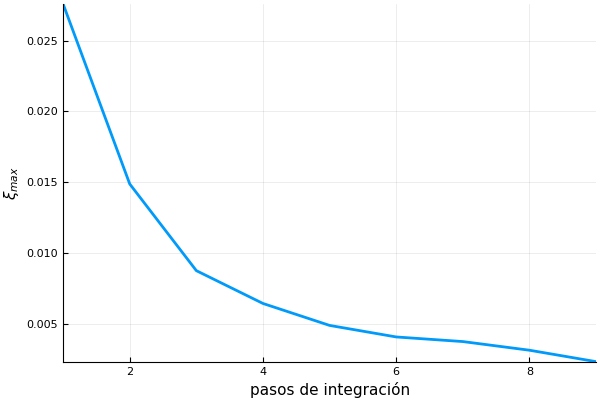
\includegraphics[width = \textwidth]{ximax_t_c3bp}
%\end{subfigure}
%%
%\begin{subfigure}{0.49\textwidth}
%	\centering
%	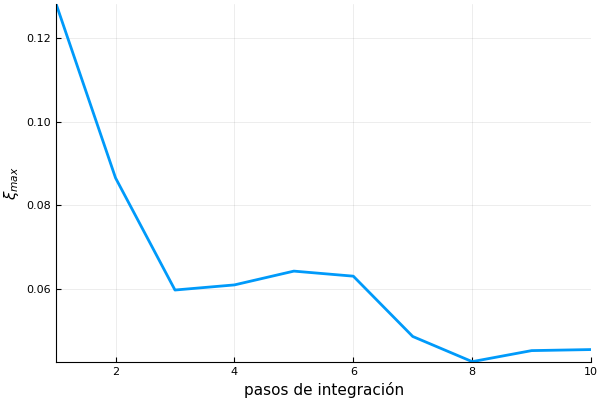
\includegraphics[width = \textwidth]{ximax_t_sp}
%\end{subfigure}
%\caption{$\xi_{max}$ en función del paso de integración del PC3C (izquierda) y el péndulo simple (derecha). Las integraciones para ambos casos fueron realizadas con una tolerancia $\epsilon_{Taylor} = 10^{-18}$, orden de la expansión $N=20$, $\epsilon_{jet} = 10^{-5}$, orden del jet $M=4$ y $10$ pasos de integración. \textit{Izquierda}: Péndulo simple con $\xo = ( \pi/2, 0)^T$. \textit{Derecha}: PC3C con $\xo = ( L_{x_1}, 0.01, 0, 0)^T$.}
%\label{fig:acc_M}
%\end{figure}
 
La segunda razón que vuelve atractivo al TJ es que propone una alternativa a los métodos de Monte Carlo. Una vez que el ćalculo está hecho, basta con evaluar los polinomios resultantes para obtener la solución en las variaciones $\delta \xo$ dadas. El problema radica en que las operaciones del álgebra polinomial son, por construcción, mucho más lentas que las operaciones numéricas estándar. Por esto, se hace un comparativo entre el TJ y el método de Monte Carlo para distinto número de evaluaciones a distintos órdenes $M$ de los jets y, como en las gráficas anteriores, se mostrará para el péndulo simple y el PC3C, con todos los demás parámetros fijos.

%FIGURE!
\begin{figure}[h!]
\centering
\begin{subfigure}{0.49\textwidth}
	\centering
	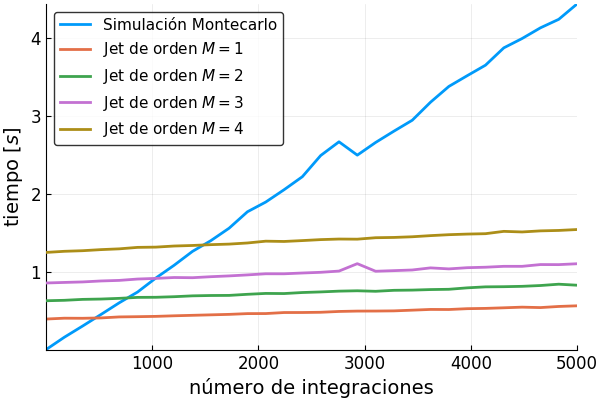
\includegraphics[width = \textwidth]{times_sp}
\end{subfigure}
%
\begin{subfigure}{0.49\textwidth}
	\centering
	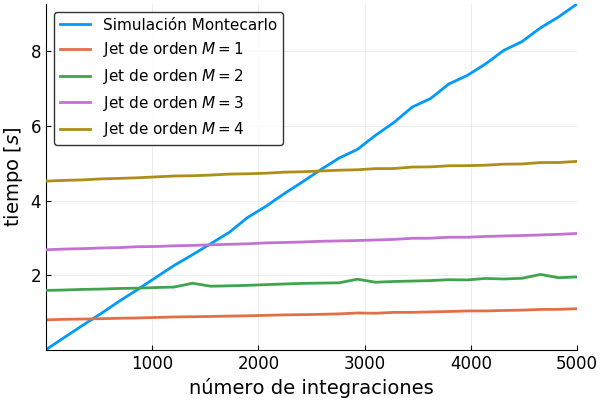
\includegraphics[width = \textwidth]{times_c3bp}
\end{subfigure}
\caption{Tiempo en segundos de cómputo en función del número de condiciones iniciales propagadas utilizando órdenes $M = \left\lbrace 1,2,3,4 \right\rbrace$ en dorado, violeta, verde y naranja, respectivamente. Las integraciones para ambos casos fueron realizadas con una tolerancia $\epsilon_{Taylor} = 10^{-18}$, orden de la expansión $N=20$ y $10$ pasos de integración que, en el caso del péndulo, corresponden a un periodo. \textit{Izquierda}: péndulo simple con condición inicial $\xo = \left(\pi/2, 0 \right)^T$. \textit{Derecha}: PC3C con condición inicial $\xo = \left(L_{4_x}, L_{4_y} + 0.01, 0, 0 \right)^T$ y $\mu = 0.012$, el parámetro Tierra-Luna.}
\label{fig:times}
\end{figure}

Se muestra en la figura \ref{fig:times} la integración de hasta $5000$ condiciones iniciales cercanas para el péndulo y el PC3C. En ambos casos se tiene un comportamiento parecido donde, para pocas integraciones, el método de Monte Carlo es más rápido que el TJ. Esto se debe a la lentitud algebráica de los polinomios operados. Sin embargo, el tiempo que demora el TJ durante toda la gráfica es casi constante para todos los órdenes; cada orden con su tiempo característico. Dicho tiempo no es exactamente constante dado que la evaluación de los polinomios sí requiere tiempo, aunque es mucho menor al de hacer una integración más. En el caso de Monte Carlo, se tiene aproximadamente una recta de pendiente positiva, lo cual es de esperarse ya que en la vecindad cada integración demora aproximadamente lo mismo. 

%FIGURE!
\begin{figure}[h!]
\centering
\begin{subfigure}{0.49\textwidth}
	\centering
	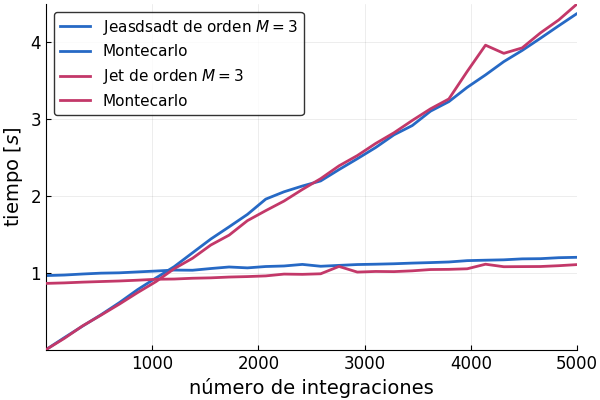
\includegraphics[width = \textwidth]{times_sp_diffx0}
\end{subfigure}
%
\begin{subfigure}{0.49\textwidth}
	\centering
	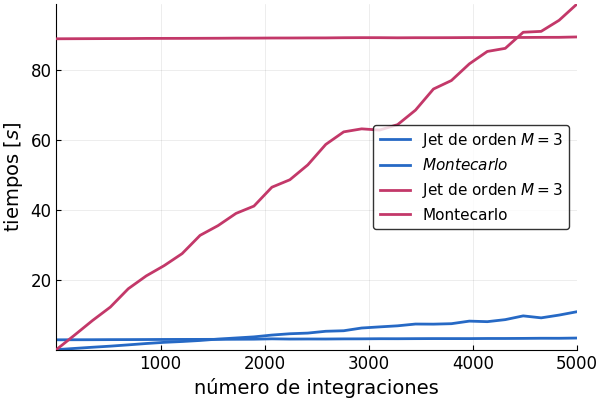
\includegraphics[width = \textwidth]{times_c3bp_diffx0}
\end{subfigure}
\caption{Tiempo en segundos de cómputo en función del número de integraciones utilizando diferentes condiciones iniciales. Ambos casos fueron realizados con una tolerancia $\epsilon_{Taylor} = 10^{-18}$, orden de la expansión $N=20$, orden del jet $M=3$ y $10$ pasos de integración que, en el caso del péndulo, corresponden a un periodo. \textit{Izquierda}: péndulo simple con condiciones inicial $\xo = \left(\pi/2, 0 \right)^T$ (azul) y $\xo = \left(15\pi/16, 0 \right)^T$ (magenta). \textit{Derecha}: PC3C con condiciones iniciales $\xo = \left(L_{4_x}, L_{4_y} + 0.01, 0, 0 \right)^T$ (azul) $\xo = \left(L_{1}, 0 + 0.01, 0, 0 \right)^T$ (magenta), con $\mu = 0.012$.}
\label{fig:times_diffx0}
\end{figure}

No todas las condiciones iniciales en el espacio fase tardan el mismo tiempo en integrarse para el mismo intervalo temporal. Por esto, se presenta la figura \ref{fig:times_diffx0}, donde se observa la dependencia de cómputo en función de la condición inicial seleccionada. El comportamiento del TJ sigue siendo casi constante aunque escala de manera considerable para las dos condiciones evaluadas. En el PC3C se hace mucho más evidente donde, para $\xo = (L_{4_x}, L_{4_x} + 0.01, 0, 0)^T$, el tiempo promedio del transporte ya evaluado es de $89.1$ segundos, mientras que para $\xo = (L_1, 0.01, 0, 0)^T$ es de tan solo $3.05$ segundos.

Finalmente, para concluir el apéndice se presentan resultados de tiempo de cómputo para algunas operaciones elementales usando el álgebra polinomial. La tabla \ref{table:times_algpoli_1} presenta la velocidad de cómputo en escala logarítmica para polinomios de dos variables pero con orden de jet variable desde $1$ hasta $32$. Como referencia, la primera fila representa el tiempo que tarda hacer la misma operación elemental con un número de punto flotante arbitrario. 

%TABLA!
\begin{table}[h!]
\centering
\begin{tabular}{c|cccc}
\toprule
     & \textbf{$\sin$} & \textbf{$\cos$} & \textbf{$\exp$} & \textbf{$\log$} \\ \cmidrule(l){1-5} 
$M=0$  & $-8.02$ & $-8.02$ & $-8.12$ & $-8.0 $ \\
$M=1$  & $-6.06$ & $-6.06$ & $-6.38$ & $-6.34$ \\
$M=2$  & $-5.87$ & $-5.88$ & $-6.18$ & $-6.13$ \\
$M=4$  & $-5.59$ & $-5.59$ & $-5.91$ & $-5.85$ \\
$M=8$  & $-5.2 $ & $-5.2 $ & $-5.5 $ & $-5.48$ \\
$M=16$ & $-4.73$ & $-4.73$ & $-5.05$ & $-5.02$ \\
$M=32$ & $-4.14$ & $-4.14$ & $-4.45$ & $-4.44$ \\ \bottomrule 
\end{tabular}
\caption{Logaritmo base $10$ del tiempo que demora hacer ciertas funciones elementales para polinomios $P(\mathbf{x}) \in \pkk{M}{2}$, es decir, polinomios en dos variables de orden $M$. $M=0$ representa la operación aritmética con un número flotante arbitrario.}
\label{table:times_algpoli_1}
\end{table}

La tabla \ref{table:times_algpoli_2}, en cambio, mantiene constante el orden del jet a $M=3$ pero cambia el numero de variables para cada operación. En todos los casos se evaluó la función elemental en la primera variable independiente del polinomio, pero tomando en cuenta que $P(\mathbf{x}) \in \pkk{3}{d}$, con $d \in \left\lbrace 1,2,3,4,5 \right\rbrace$. 

%TABLA!
\begin{table}[h!]
\centering
\begin{tabular}{c|cccc}
\toprule
     & \textbf{$\sin$} & \textbf{$\cos$} & \textbf{$\exp$} & \textbf{$\log$} \\ \cmidrule(l){1-5} 
 $\#_{vars} = 0$ & $-8.02$ & $-8.02$ & $-8.12$ & $-8.00$ \\
 $\#_{vars} = 1$ & $-5.68$ & $-5.68$ & $-5.98$ & $-5.92$ \\
 $\#_{vars} = 2$ & $-5.60$ & $-5.59$ & $-5.90$ & $-5.84$ \\
 $\#_{vars} = 3$ & $-5.56$ & $-5.56$ & $-5.87$ & $-5.82$ \\
 $\#_{vars} = 4$ & $-5.53$ & $-5.53$ & $-5.84$ & $-5.80$ \\
 $\#_{vars} = 5$ & $-5.47$ & $-5.47$ & $-5.78$ & $-5.74$ \\ \bottomrule 
\end{tabular}
\caption{Logaritmo base $10$ del tiempo que demora hacer cada operación elemental para polinomios $P(\mathbf{x}) \in \pkk{3}{d}$, es decir, polinomios en $d$ variables de orden $M = 3$. $\#_{vars}=0$ representa la operación aritmética con un número flotante arbitrario.}
\label{table:times_algpoli_2}
\end{table}

Todos los cálculos aquí presentados fueron realizados en serie, con un CPU Intel\textregistered  Core\texttrademark  i7-7700HQ @ 2.80GHz $\times$ 8. El lenguaje utilizado para el cálculo es \href{julialang.org}{\textsf{Julia}}, versión $0.6.0$. El álgebra polinomial es operado con el paquete \textsf{TaylorSeries} \cite{TaylorIntegration} versión $0.7.2$ y la integración del transporte de jets es realizada con el paquete \textsf{TaylorIntegration} \cite{TaylorIntegration} versión $0.2.1$.